\section{Methods}

\subsection{Design requirements from human physiology}

The jaw makes essential contributions to the chewing process such as generating the forces required to break down food, controlling the lower mandible motion
and giving sensory feedback. A robotic jaw should therefore be able to mimic these functions as closely as possible.
As this is the first iteration of the chewing robot, we focus on force generation and range of motion, while sensory feedback and other functions can be added in future iterations.
The design requirements are based on the literature and the human jaw anatomy and physiology, as summarized in Table~\ref{tab:functional_criteria}.
Note that the jaw's speed is not a design requirement as food can be effictively chewed even at slow speeds.

\begin{table}[H]
  \centering
  \begin{tabular}{@{}L{4.2cm}L{6.4cm}L{4.2cm}@{}}
    \toprule
    \textbf{Quantity} & \textbf{Values reported in the literature} & \textbf{Design requirement} \\
    \midrule
    Degrees of freedom (DoF) 
      & 6 DoF: 3 translational (X, Y, Z) and 3 rotational (roll, pitch, yaw) \cite{6dof}
      & 6 DoF \\[2pt]
    \hline
    Vertical (compressive) bite force $F_{z}$ 
      & $600$ N chewing force in healthy adults \cite{chewing_force},\; $1243$ N maximum clenching force \cite{max_clenching_force}
      & $800$ N \\[2pt]
    
    \hline

    Lateral force $F_{x}$ 
      & $-72$ N (left) to $+53$ N (right) during maximal biting \cite{shear_force}
      & $\pm100$ N \\[2pt]
    \hline

    Anterior–posterior force $F_{y}$ 
      & $-10$ N (posterior) to $+30$ N (anterior) \cite{shear_force}
      & $\pm50$ N \\[2pt]
    \hline

    Mandibular motion range 
      & $14$ mm lateral shift, $11$ mm protrusion, $61$ mm mouth opening in healthy adults \cite{range_motion_required}
      & $\pm20$ mm (X, Y);\;\; $0$–$70$ mm (Z) \\[2pt]
  \bottomrule
  \end{tabular}
  \caption{Functional design requirements.}
  \label{tab:functional_criteria}
\end{table}


\subsection{Mechanical design}
\begin{itemize}
    \item choosing the dimensions of the stewart platform based on the size of the actuators + working space of the robot
    \item choice of structure/material to hold upper jaw to be rigid enough to not deform under the forces applied by the actuators 
    \item 3 axis load cells to measure the force applied by the jaw
    \item so far 3d printed teeth/jaw but to be changed in the future
\end{itemize}

The first major design decision was how to achieve 6 degrees of freedom (DoF) for jaw motion. In the field of robotic mastication, two common approaches 
are used. The first is a biomechanically inspired design using linear actuators \cite{ChewingRobotLinearActuator} or combinations of actuated cables and 
springs \cite{ChewingRobotGums} to replicate muscle behavior. The second is a Stewart platform \cite{BristolChewingRobot}—a widely used 6-DoF parallel mechanism, often seen in 
motion simulators. See Figure~\ref{fig:stewart_platforms} for a visualization of the two approaches.

For this project, we chose the Stewart platform approach. Its well-defined kinematics and ease of control make it particularly suitable for our goal of 
replicating recorded human chewing motion. Because our control strategy is based on reproducing real motion trajectories, having a platform with 
straightforward inverse kinematics is a key advantage.

Stewart platforms generally come in two configurations: one based on rotary servo motors and one based on linear actuators, see Figure~\ref{fig:stewart_platforms}. 
We selected the linear actuator design for several reasons. It offers more efficient force transmission, a simpler kinematic model, and greater structural 
rigidity—all important factors when attempting to reproduce the forces involved in human chewing.

% 3 pictures side by side of the two approaches
\begin{figure}[H]
\centering
\begin{minipage}{.3\textwidth}
  \centering
  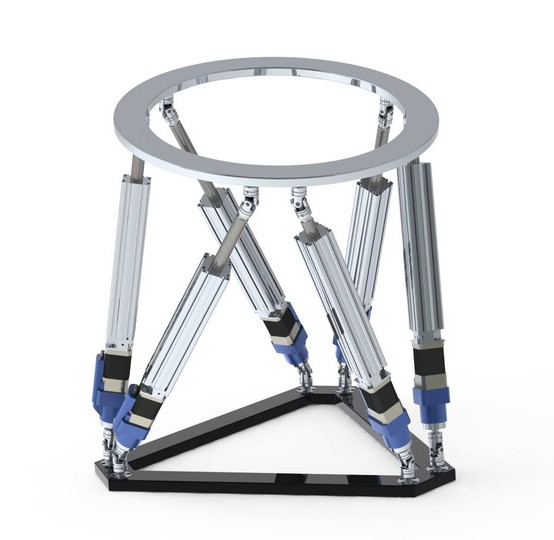
\includegraphics[height=4.6cm]{figures/linear_stewart_platform_2.jpg}
  \subcaption{}
  \label{fig:linear_stewart_platform}
\end{minipage}
\begin{minipage}{.3\textwidth}
  \centering
  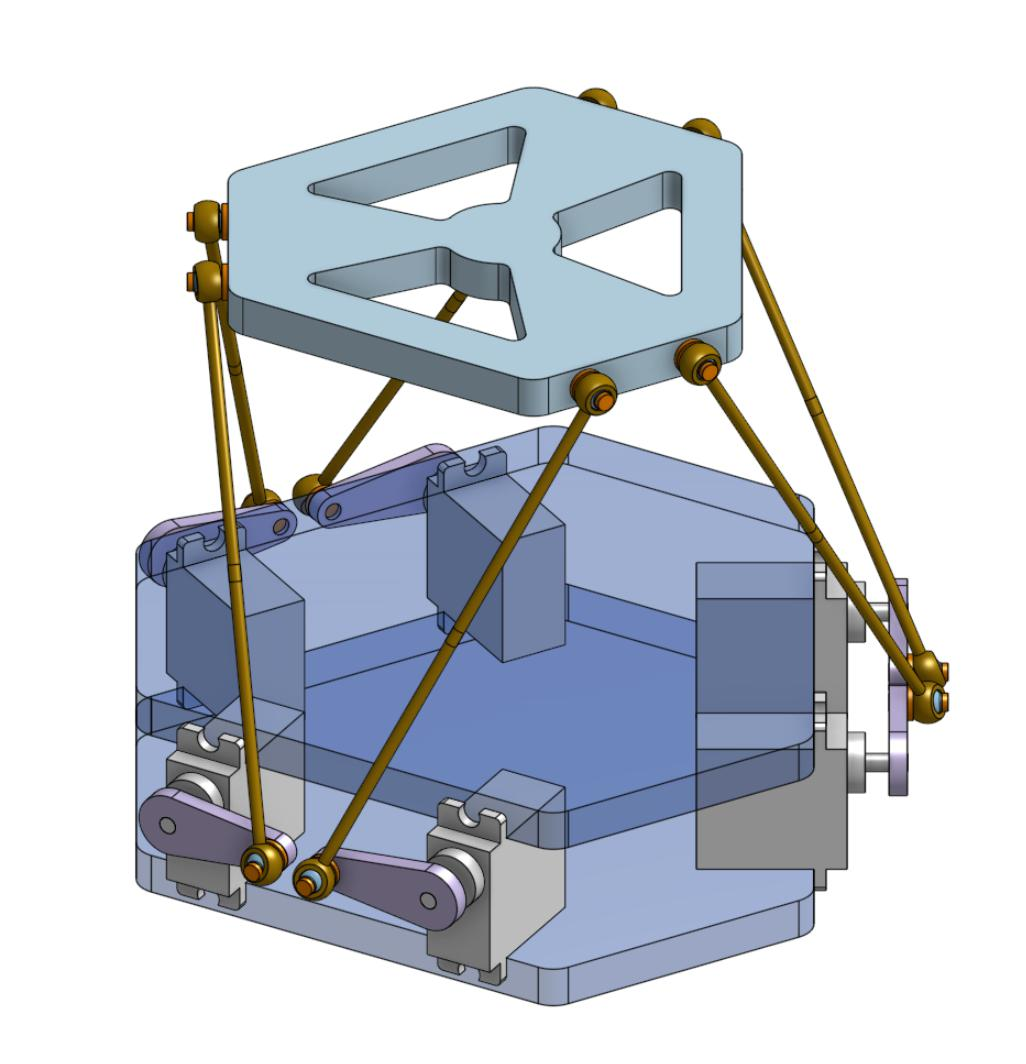
\includegraphics[height=4.6cm]{figures/rotary-stewart-plateform.jpg}
  \subcaption{}
  \label{fig:rotary_stewart_platform}
\end{minipage}
\begin{minipage}{.3\textwidth}
  \centering
  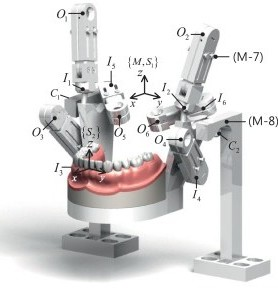
\includegraphics[height=4.6cm]{figures/6dof_jaw_cad.jpg}
  \subcaption{}
  \label{fig:biomechanically_inspired_design}
\end{minipage}
\caption{(a) Linear actuator-based jaw design. (b) Rotary servo motor-based Stewart platform. (c) Biomechanically inspired design\cite{ChewingRobotLinearActuator}.}
\label{fig:stewart_platforms}
\end{figure}

The platform's dimensions were determined based on actuator specifications, desired jaw range of motion, and the working space required. The working space 
refers to the overall range of jaw motion and is defined by functional requirements summarized in Table~\ref{tab:functional_criteria}. Based on findings 
in \cite{StewartPlatformWorkspace}, we prioritized achieving the necessary vertical range of motion, knowing that sufficient horizontal range would follow.

Assuming a minimum actuator mounting angle of 45° to the horizontal, the minimum required stroke length is calculated as:
\begin{equation}
l_{\text{min}} = \frac{z_{\text{max}} - z_{\text{min}}}{\sin(45^\circ)} = \frac{70\,\text{mm}}{\sin(45^\circ)} \approx 99\,\text{mm}
\end{equation}

To meet the minimum vertical force requirement of 800 N, each actuator must provide:
\begin{equation}
F_{\text{min}} = \frac{F_{z,\text{min}}}{6 \cdot \sin(45^\circ)} = \frac{800\,\text{N}}{6 \cdot \sin(45^\circ)} \approx 189\,\text{N}
\end{equation}

With this minimum actuator force, we estimate the lateral (shear) and front-back force capacities as:
\begin{equation}
F_{x} \approx 2 \cdot \cos(45^\circ) \cdot F_{\text{min}} + 4 \cdot \cos(45^\circ) \cdot \sin(30^\circ) \cdot F_{\text{min}} \approx 534\,\text{N} \gg 100\,\text{N}
\end{equation}
\begin{equation}
F_{y} \approx 4 \cdot \cos(45^\circ) \cdot \cos(30^\circ) \cdot F_{\text{min}} \approx 462\,\text{N} \gg 50\,\text{N}
\end{equation}

These calculations show that ensuring the vertical force requirement is met also guarantees that shear forces in the x and y directions will exceed 
their respective targets.

Since speed is not a strict requirement for this prototype, we prioritized force over velocity when selecting actuators. Position feedback is necessary 
for closed-loop control, as we use inverse kinematics to compute actuator positions based on the desired platform pose.

We selected the PA-14P-4-50 linear actuator, which meets both stroke and force requirements as seen in table \ref{tab:actuator_spec}.
%spec of actuator
\begin{table}[H]
\centering
\begin{tabular}{@{}p{3cm} p{3cm}@{}}
\toprule
\textbf{Parameter} & \textbf{Value}\\
\midrule
Stroke length & 101 mm \\
Max force & 222.4 N \\
Speed (no load) & 28 mm/s \\
Speed (full load) & 21 mm/s \\
Position feedback & Potentiometer \\
\bottomrule
\end{tabular}
\caption{PA-14P-4-50 specifications.}
\label{tab:actuator_spec}
\end{table}



\subsection{Control}

%The control layer combines a high-speed microcontroller, a modular C++ codebase, and classical PI loops to deliver real-time motion of 
%the Stewart platform.  Figure~\ref{fig:code_structure} gives the software context, while the full electronics schematic is shown in 
%Fig.~\ref{fig:elec_schematic}.

\subsubsection{Hardware (electronics)}
A Teensy~4.1 (600 MHz ARM Cortex-M7, single-precision FPU) executes the control loop.% at \SI{100}{\hertz}. %? %todo: add ref for the freq/reason
Its key peripherals are:  
\begin{itemize}[nosep]
    \item three \SI{12}{\ampere} dual DC motor drivers (DF Robot) controlling the six linear actuators;
    \item six analogue inputs reading potentiometer position feedback from the linear actuators;
    \item three transmitters for the load cells mounted on top of the maxilla;
    \item an on-board micro-SD slot used for trajectory files and calibration data.
\end{itemize}
A \SI{12}{\volt} AC/DC brick powers the actuators directly; the user's computer supplies \SI{5}{\volt} to the Teensy, which in 
turn sources the \SI{3.3}{\volt} logic rails for the motor drivers and load-cell transmitters.
The full electronics schematic is shown in Fig.~\ref{fig:elec_schematic}.

\begin{figure}[H]
\centering
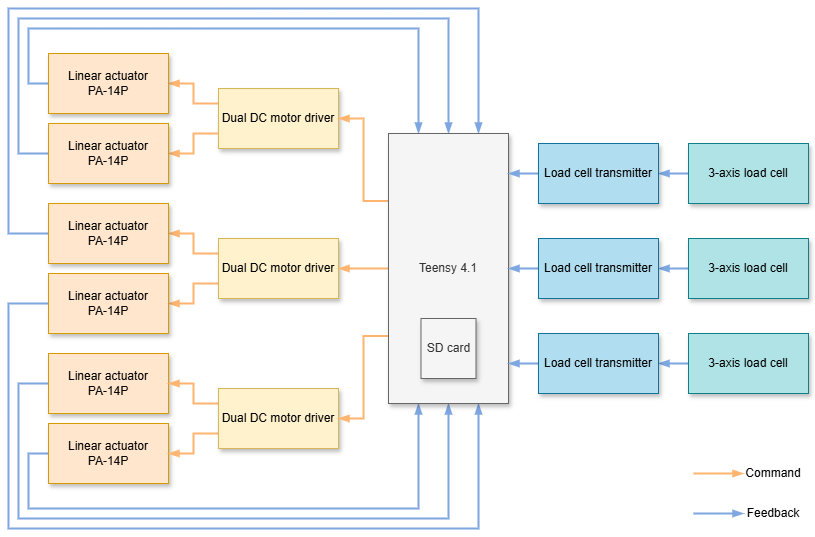
\includegraphics[width=\textwidth]{figures/elec_schematic.drawio.png}
\caption{Electronics schematic.}
\label{fig:elec_schematic}
\end{figure}

\subsubsection{Software architecture}
The central class \texttt{RobotController} maintains the finite-state machine in Fig.~\ref{fig:state_machine} and manages two
 modules:  
\begin{itemize}[nosep]
    \item \texttt{StewartPlatform}: inverse kinematics, trajectory interpolation, and low-level actuator commands;
    \item \texttt{ForceSensing}: continuous load-cell acquisition and filtering;
\end{itemize}
The controller is designed to be modular, allowing for easy addition of new modules such as a tongue or saliva module in the future.
The three controller states are:
\begin{enumerate}
    \item \textbf{Stop} – return to home pose; reload trajectory if the user selects a new file;
    \item \textbf{Calibrate} – user can manually change the initial $(x,y,z)$ position via the GUI;
    \item \textbf{Move} – replay the selected trajectory.
\end{enumerate}
A lightweight Python GUI on the host PC issues high-level commands, such as state changes, and plots sensor data.  

    

\begin{figure}[H]
\centering
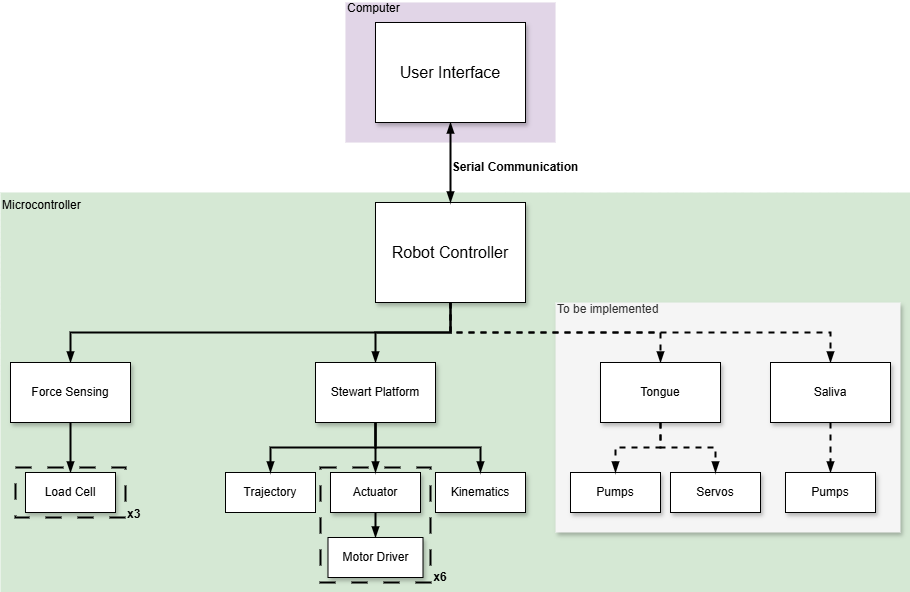
\includegraphics[width=\textwidth]{figures/code_structure.drawio.png}
\caption{Overall code structure.}
\label{fig:code_structure}
\end{figure}


\begin{figure}[H]
\centering
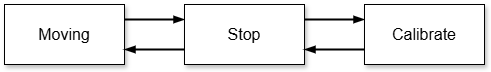
\includegraphics[width=0.6\textwidth]{figures/state_machine.drawio.png}
\caption{Robot controller state machine.}
\label{fig:state_machine}
\end{figure}

\subsubsection{Position control}

The Stewart Platform follows a 3D trajectory (x, y, z, roll, pitch, yaw) from a .csv file on the micro-SD card.
See section \ref{sec:motion-capture} for details on the recording protocol and data processing.
Each pose is defined by its position ${\bf t}=(x,y,z)$ and orientation given by the Euler angles $(\phi,\theta,\psi)$,
 which are the roll, pitch, and yaw angles respectively.
The trajectory is then linearly interpolated with a fixed time step chosen by the user.

\paragraph{Inverse kinematics}
For each pose in the trajectory, \texttt{Kinematics} computes the lengths of the six linear actuators that will achieve 
the desired pose of the platform, i.e. the inverse kinematics. To do so, we first compute the standard rotation matrix 
$R(\phi,\theta,\psi)$ for the Euler angles, which is defined as the product of three rotation matrices about 
the $Z$, $Y$, and $X$ axes:
\[
R(\phi,\theta,\psi) = R_Z(\psi) R_Y(\theta) R_X(\phi) =
\begin{pmatrix}
\cos\psi & -\sin\psi & 0 \\
\sin\psi & \cos\psi & 0 \\
0 & 0 & 1
\end{pmatrix}
\begin{pmatrix}
\cos\theta & 0 & \sin\theta \\
0 & 1 & 0 \\
-\sin\theta & 0 & \cos\theta
\end{pmatrix}
\begin{pmatrix}
1 & 0 & 0 \\
0 & \cos\phi & -\sin\phi \\
0 & \sin\phi & \cos\phi
\end{pmatrix}
\]

The platform joints ${\bf p}_i$, $i$ being the actuator index, are then rotated about a fixed point ${\bf c}$, 
which is the front of the gnathion, and translated by the user-defined home position ${\bf t}=(x,y,z)$, 
resulting in the world coordinates of the platform joints:
\[
{\bf w}_i = R\bigl({\bf p}_i-{\bf c}\bigr)+{\bf c}+{\bf t}.
\]

Finally, the actuator length is the Euclidean distance to the fixed base joint ${\bf b}_i$:
\[
\ell_i = \lVert {\bf w}_i-{\bf b}_i\rVert_2.
\]

\paragraph{PI controller}
For each actuator, its desired length is sent to a PI position controller, see Figure~\ref{fig:actuator_pi}.
To minimize the noise of the potentiometer feedback, we apply a low-pass filter averaging the last 10 samples.
\begin{figure}[H]
\centering
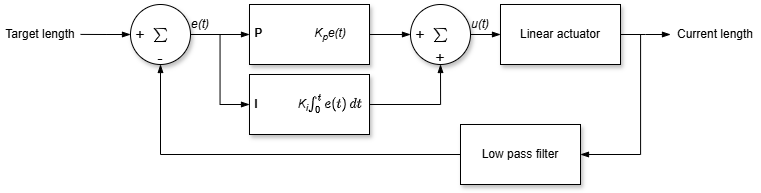
\includegraphics[width=\textwidth]{figures/actuator_pi.drawio.png}
\caption{Position PI controller for the linear actuators.}
\label{fig:actuator_pi}
\end{figure}

\subsection{Data acquisition and processing}
\label{sec:motion-capture}

\paragraph{Subjects.} 
Two healthy adult volunteers (author and project supervisor) participated in this pilot recording. Owing to time constraints and the exploratory 
nature of the study, no additional subjects were recruited.

\paragraph{Motion-capture acquisition.}
Mandibular motion was recorded with a five-camera OptiTrack system sampling at 120 Hz.
Four reflective markers arranged in a square were attached to the forehead and served as a head-fixed reference frame.
A second set of three markers forming a triangle was placed on the gnathion.
Two additional lip markers were recorded but later discarded because a single marker cannot encode orientation. \cite{motion_capture_adult,motion_capture_children}

The subject then performed the motion sequences listed in Table~\ref{tab:recording-protocol}. Each frame was saved by Motive as a \texttt{.csv} file that contains
the 3-D marker positions (in millimetres) and the orientation of each marker set as quaternions. The calibrated volume had a residual error of $0.3\,$mm.
% TODO: insert a photograph of the marker placement

\begin{table}[H]
  \centering
  \small                                   
  \renewcommand{\arraystretch}{1.1}  
  \begin{tabularx}{\textwidth}{@{} c l l @{}}      
    \toprule
    \textbf{Food} & \textbf{Motion} & \textbf{\textit{Optional:} Duration} \\
    \midrule
    % ---------- Empty mouth block ----------
    Empty mouth & 20$\times$ open–close cycles                 & —     \\[1pt]
    \midrule
    % ---------- Chewing-gum block ----------
    \multirow{5}{*}{\parbox[c]{3.2cm}{\centering Chewing gum\\(Xylit-Pro,\\\emph{Excitemint})}}
      & Random side chewing                                    & 2 min \\[1pt]
      & Right-side chewing                                     & 1 min \\[1pt]
      & Left-side chewing                                      & 1 min \\[1pt]
      & Front-teeth-only chewing                               & 1 min \\ 
    \midrule
    % ---------- Biscuit block ----------
    \multirow{5}{*}{\parbox[c]{3.2cm}{\centering Biscuits\\(Bretzeli, \emph{Kambli})}}
      & random chewing                                    & — \\[1pt]
      & front-teeth chew → right-side chew                & — \\[1pt]
      & front-teeth chew → left-side chew                  & — \\[1pt]
      & \textit{fast} random chewing                      & — \\[1pt]
      & \textit{slow} random chewing                       & — \\
    \bottomrule
  \end{tabularx}
  \caption{Recording protocol. \textit{Notes:}  
  For chewing-gum trials the first run began with an unchewed piece and the same gum was kept for all subsequent motions.  
  For biscuit trials each run started with an empty, closed mouth; the subject then placed a biscuit, chewed as instructed, and swallowed.}
  \label{tab:recording-protocol}
\end{table}

\paragraph{Data processing.}
To reduce the noise, we apply a 4th-order butterworth filter to the data. The cutoff frequency is set to 6Hz, as human mastication frequency is around 1Hz to 2Hz %\cite{chewing_frequency} TODO: find paper
. \\
The data is then transformed to the head reference frame using rotation matrices. 







